
\begin{figure}
\begin{center}
    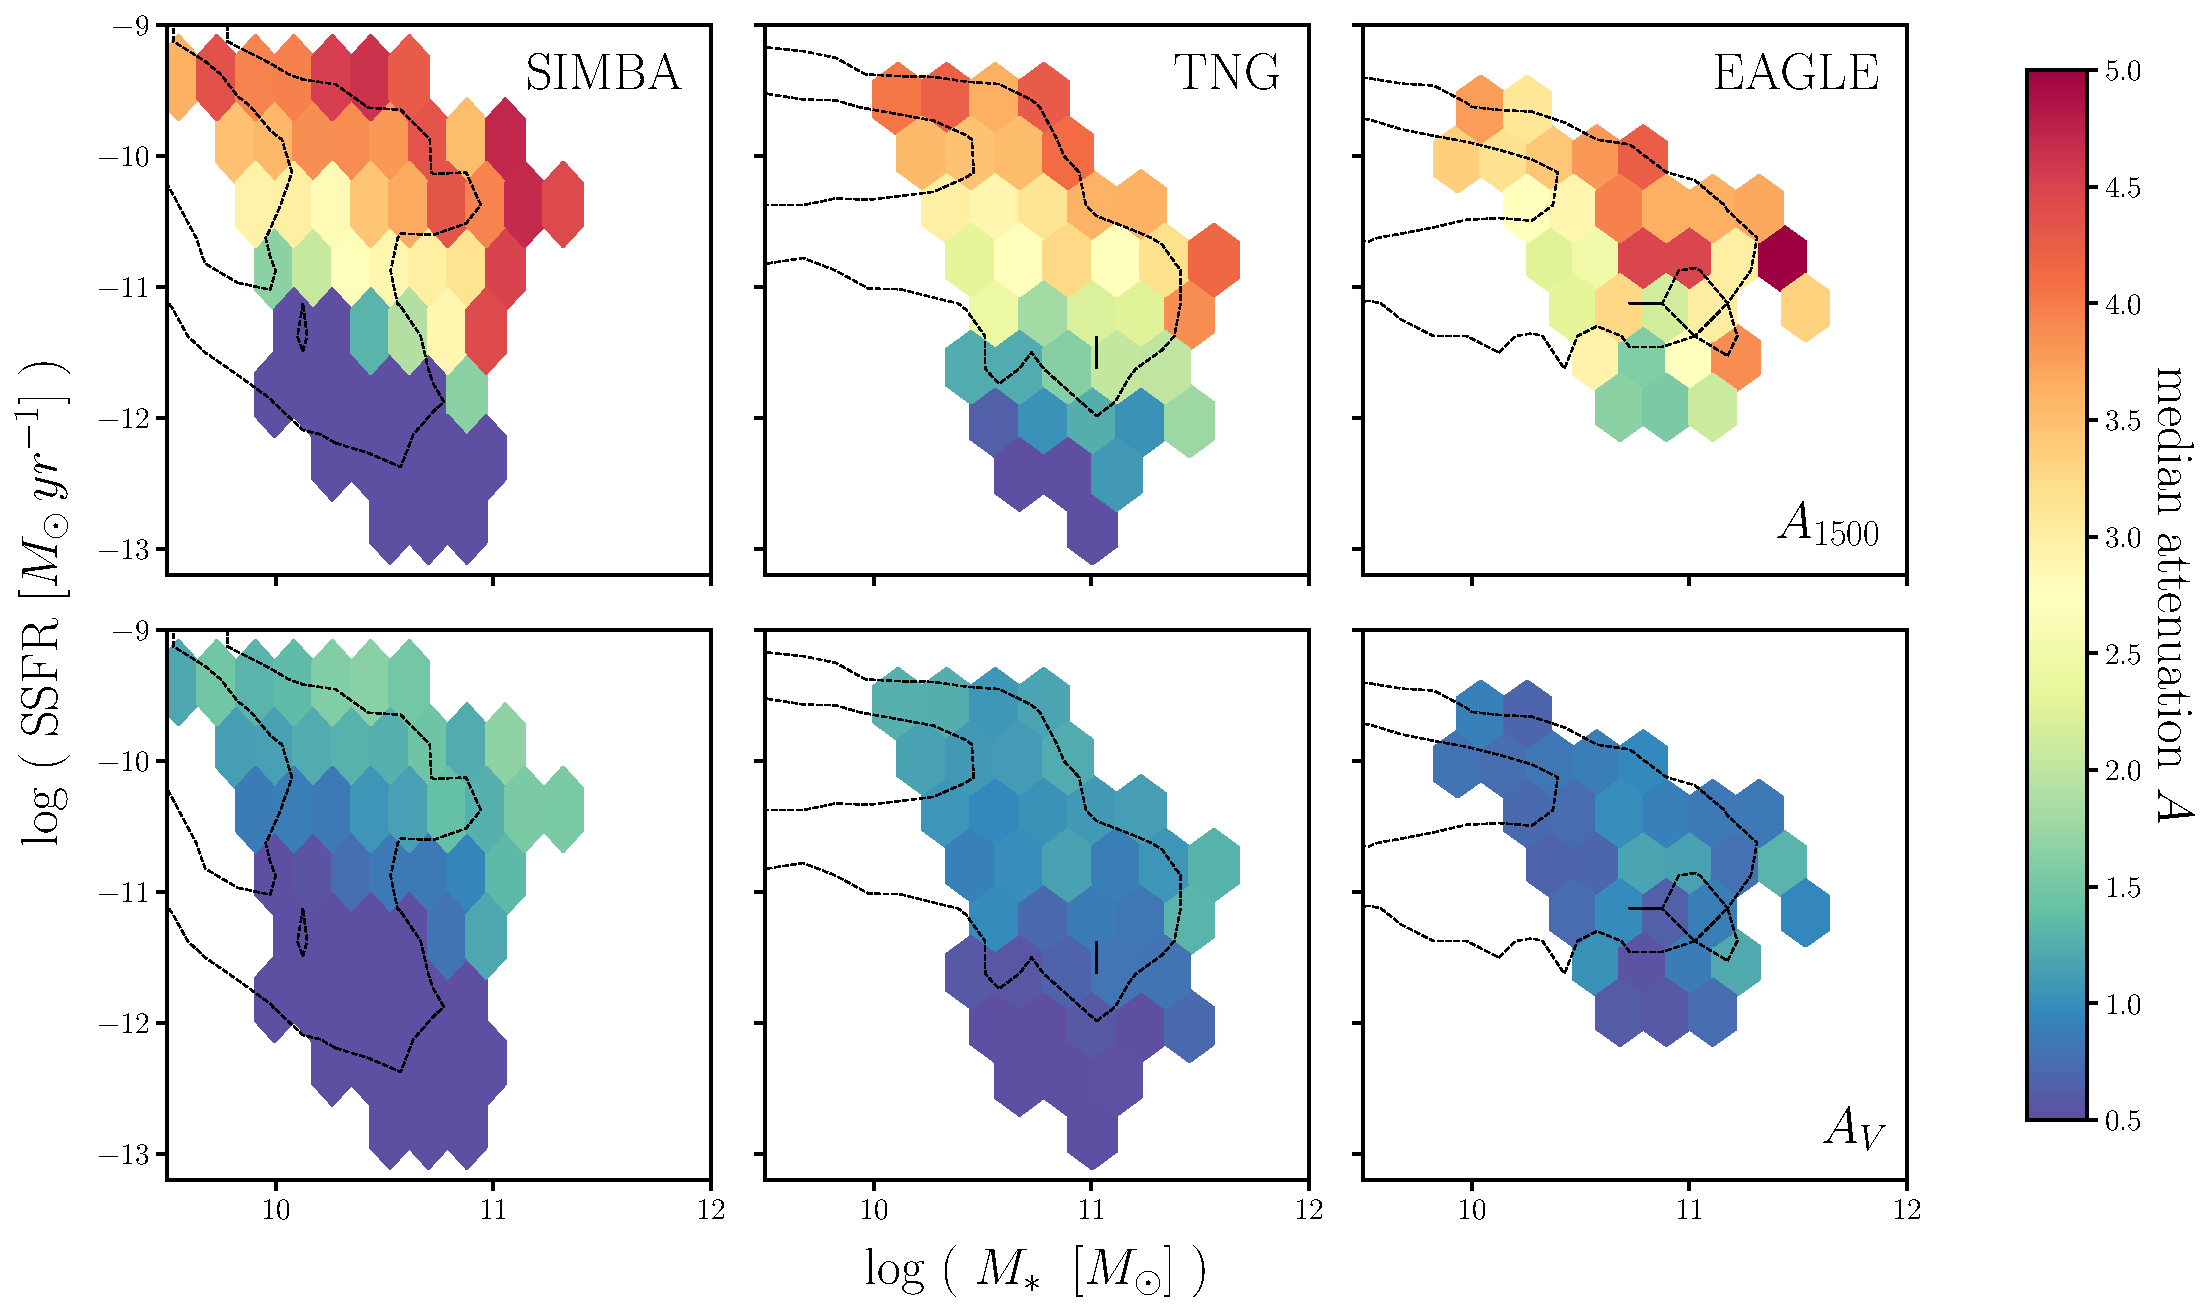
\includegraphics[width=0.9\textwidth]{figs/abc_av_mssfr.pdf}
    \caption{\label{fig:avmsfr}
    \chedit{ 
        $M_*$ and $\ssfr$ dependence of dust attenuation at $1500 \AA$
        ($A_{1500}$; top) and at $5500\AA$ ($A_{V}$ bottom) predicted by the
        \eda~for TNG (left) and EAGLE (right). The colormap in each hexbin 
        represents the median attenuation for all simulated galaxies in the
        bin (right color bar). We only include bins with more than 10 galaxies that
        satisfy our $M_r < -20$ completeness limit.
        Overall, TNG and EAGLE galaxies with higher $M_*$ have higher dust
        attenuation --- consistent with the literature.
        Furthermore, since previous works have primarily focused on star-forming
        galaxies, the \eda~provides new insight into the \ssfr dependence of
        dust attenuation: simulated galaxies with higher $\ssfr$ have steeper
        attenuation curves. 
    }
    }
\end{center}
\end{figure}

\subsection{The Galaxy -- Dust Connection}  
\chedit{
    With the \eda~framework, we can also shed light on the connection between
    the physical properties of the simulated galaxies and dust attenuations.
    In our \eda~prescription, we included a flexible $M_*$ and $\ssfr$ dependence in both the
    amplitude and slope of the attenuation curve~(Eqs~\ref{eq:tauv}
    and~\ref{eq:delta}). 
    Hence, we can reveal the $M_*$ and $\ssfr$ dependence of dust attenuation
    through both the \eda~parameter constraints (Figure~\ref{fig:abc}) and the
    predicted attenuation curves. 
}


\chedit{
    Focusing first on the amplitude of dust attenuation, we find that TNG has
    little $M_*$ dependence in $\tau_V$: 
    $\mtaum = 0.14\substack{+0.64 \\ -0.58}$. 
    EAGLE has a more significant positive $M_*$ dependence:
    $\mtaum = 0.53\substack{+0.36 \\ -0.36}$.
    Though neither TNG nor EAGLE has a strong dependence, $V$-band dust
    attenuation is higher for more massive galaxies.  
    Meanwhile, we find significant $\ssfr$ dependences in both TNG 
    ($\mtaus = -0.42\substack{+0.2 \\ -0.18}$)
    and EAGLE
    ($\mtaus = -0.24\substack{+0.22 \\ -0.19}$): galaxies with higher $\ssfr$
    have lower $V$-band dust attenuation. 
    For the slope of the dust attenuation, we find some $M_*$ dependence in
    both TNG 
    ($\mdeltam = -0.36\substack{+0.23\\-0.19}$)
    and EAGLE
    ($\mdeltam = -0.2\substack{+0.16\\-0.16}$). 
    More massive galaxies have slightly steeper attenuation curves. 
    We also find significant $\ssfr$ dependence in both TNG 
    ($\mdeltas = -0.55\substack{+0.08 \\ -0.08}$)
    and EAGLE
    ($\mdeltas = -0.43\substack{+0.08 \\ -0.08}$).
    Galaxies with higher $\ssfr$ have steeper attenuation curves.
}

\chedit{
    We take a closer look at the $M_*$ and $\ssfr$ dependence of the
    attenuation curve in Figure~\ref{fig:avmsfr}. We present dust attenuation
    at $1500\AA$ ($A_{1500}$; top) and $5500\AA$ ($A_V$; bottom) as a function
    of $\log M_*$ and $\log \ssfr$ predicted by the \eda~for TNG (left) and
    EAGLE (right). For each hexbin, the colormap represents the median
    attenuation for all simulated galaxies in the bin. We only include
    bins with more than 10 galaxies that satisfy our $M_r < -20$
    completeness limit. 
    In each of the panels, we find that TNG and EAGLE galaxies with higher
    $M_*$ have higher dust attenuation --- consistent with the literature.
    \cite{burgarella2005}, for instance, found significant positive $M_*$
    dependence in $FUV$ attenuation in NUV-selected and FIR-selected samples. 
    \cite{garn2010} and \cite{battisti2016} also find higher attenuation in
    more massive SDSS star-forming galaxies. 
    Most recently, \cite{salim2018} find higher $V$ and $FUV$ attenuation for
    more masssive star-forming galaxies in GSWLC2. 
}

\chedit{ 
    For the $\ssfr$ dependence, we find that galaxies with higher $\ssfr$ have
    higher $A_{1500}$ (top) but lower $A_V$ (bottom). 
    The opposite $\ssfr$ dependence in $A_{1500}$ versus $A_V$ is a result of
    the significant $\ssfr$ dependence on the slope of the attenuation curve. 
    Galaxies with higher $\ssfr$ have significantly steeper slopes so even
    though they have lower $A_V$, they have higher $A_{1500}$. 
    At the lowest $\ssfr$ end, quiescent galaxies in TNG and EAGLE have nearly
    flat attenuation curves. 
    Since observations have only focused on star-forming galaxies due to the
    difficult in measuring dust attenuation in quiescent galaxies, the
    \eda~predicitons provide new insight into the $\ssfr$ dependence of dust attenuation. 
    In summary, from the \eda~predictions, we find that \emph{TNG and EAGLE
    galaxies with higher $M_*$ require overall higher dust attenuation and
    galaxies with higher $\ssfr$ require steeper attenuation curves}.
} 

